\section{Introduction}
Economic narratives often specify a pathway from a macroeconomic development to an asset price. Turning such a narrative into a decision requires more than predicting a market regime. The question must specify what changes, which outcome is measured, the time horizon, the information available at the decision, and the assumptions under which the effect can be recovered from observations. A latent-state label by itself supplies none of these guarantees.

The Causal Macro Transmission Framework (CMTF) organizes this boundary between mechanism proposals and decision eligibility. It continues the author's earlier conceptual note \citep{olapade2026agentic}, while narrowing the empirical contribution to an executable routing contract and a controlled synthetic diagnostic. A neural component may propose a mechanism or forecast; a symbolic record specifies its evidence status and applicability. The implementation tested here consumes declared records. It does not use a language model to establish identification, learn an economic causal graph, or verify the truth of an assumption.

We distinguish three questions. Is a causal effect identified under a declared model? Can the execution system infer the current regime reliably? Does a proposed action match the direction, horizon, and information vintage of its supporting evidence? Failure in one cannot generally be repaired by success in another. The synthetic study isolates the first two; the router implements a minimal contract for declared evidence. Neither is presented as a full deployed neuro-symbolic trading system.

Our main finding is a reversal: filtered routing improves coefficient recovery under the nominal observation mechanism, but becomes worse than pooled adjustment after the observation-to-regime relationship is reversed. A second finding is that oracle knowledge of the regime does not remove hidden-confounding bias. Together these motivate explicit failure states rather than a single undifferentiated confidence score.

\section{Positioning and contribution}
Mixture-of-experts systems combine specialist outputs using input-dependent weights \citep{jacobs1991}. Weighting addresses which prediction to use; causal identification addresses whether the target effect is recoverable from the assumed graph and observed data. These are different operations. DoWhy explicitly separates modeling, identification, estimation, and refutation \citep{sharma2020}. CMTF adopts this separation as an interface constraint rather than introducing a replacement identification calculus.

Selective prediction permits a system to decline an output when a selection criterion is not met \citep{geifman2019selectivenet}. Our router's abstention is a deterministic contract outcome when no record passes the declared checks. It does not learn a calibrated risk--coverage trade-off. Here coverage means the fraction of cases receiving an output, and risk means the error on those retained cases; neither is measured on a real decision dataset in this study.

The original macro-to-asset framing supplies a use case, not evidence that a particular economic graph is correct. The present contribution comprises a precise record-to-routing interface, executable contract checks, and a four-scenario diagnostic with a known data-generating process. Standard regression and filtering are used to expose failure modes, not claimed as new estimators.

\section{Evidence records and routing}
\subsection{A declared causal question}
Let $X$ be a treatment variable, $Y$ an outcome, and $C$ a set of pre-treatment context variables. A treatment is the variable whose value is hypothetically changed; a context variable is observed before that change. For values $x_1,x_0$ and context $c$, a possible query is
\begin{equation}
 \tau(c)=\mathbb{E}[Y\mid\operatorname{do}(X=x_1),C=c]
 -\mathbb{E}[Y\mid\operatorname{do}(X=x_0),C=c].
\end{equation}
The scalar $\tau$ (tau) is a defined causal contrast. $\mathbb{E}$ denotes an expected value, or average under the specified distribution. The operator $\operatorname{do}$ denotes intervention: set $X$ externally rather than merely select observations with a certain $X$. The vertical bar means conditioning. This definition does not establish that the contrast can be estimated from the available data.

An evidence record should specify the query, graph version, identification argument, estimator version, units, horizon, availability time, expiry, and unresolved assumptions. An execution-state estimate is kept distinct from the pre-treatment context used for identification. Conditioning on a variable caused by the treatment can change or bias the target; a convenient state feature must not automatically be used as a causal adjustment variable.

\subsection{The implemented contract}
The reference implementation stores, for each expert $k$, a unique identifier; direction $d_k\in\{-1,0,1\}$; score $s_k$; response $r_k$; nonnegative penalty $p_k$; availability and expiry times; a declared identification flag; and a provenance string. Scores, responses, and penalties are finite scalar inputs. They are assumed to be on a compatible dimensionless scale in this demonstration. Real effects with different units or horizons require explicit conversion before aggregation.

At decision time $t$, the router rejects nonfinite values, invalid directions, negative penalties, missing provenance, records declared unidentified, and records unavailable or expired at $t$. A duplicate expert identifier raises an error. The identification flag is supplied by the caller; checking it does not prove identification. The richer graph, units, horizon, and diagnostic checks described above are an interface specification, not fully implemented validators.

For eligible expert set $\mathcal{K}_t$, the chosen logit and normalized weight are
\begin{align}
 \ell_k&=s_k+d_kr_k-p_k,\\
 w_k&=\frac{\exp(\ell_k-m)}{\sum_{j\in\mathcal{K}_t}\exp(\ell_j-m)},\qquad
 m=\max_{j\in\mathcal{K}_t}\ell_j.
\end{align}
Here $\ell$ (ell) is a scalar routing score, $w_k$ is a nonnegative weight, $\exp$ is the exponential function, and $j$ indexes eligible experts. The set $\mathcal{K}_t$ contains only records that passed the contract. Subtracting the maximum $m$ leaves the normalized ratios unchanged while preventing exponential overflow. The weights sum to one. If the eligible set is empty, the output is an abstention record with reasons; the denominator is never evaluated.

The direction term rewards alignment with the signed response. For example, with score 0.2, response $-0.8$, and penalty 0.1, a long proposal has logit $0.2-0.8-0.1=-0.7$, while a short proposal has logit $0.2+0.8-0.1=0.9$. With only these two eligible experts, their weights are approximately 0.168 and 0.832. A future-dated proposal is rejected even if its numerical score is very large. The example explains contract behavior; these numbers are not calibrated trading preferences.

The algorithm scans records once for validation, computes eligible logits, and normalizes them. A dictionary stores rejection reasons keyed by expert identifier, and another stores eligible weights. For $K$ records, both time and storage grow linearly, written $O(K)$: doubling the number of records approximately doubles the work and retained entries. Portfolio constraints and order execution occur after routing and are outside this demonstration.

\section{Synthetic diagnostic}
\subsection{Data-generating process}
Each dataset contains 3,000 sequential observations: 2,000 training and 1,000 test. Let $S_t\in\{0,1\}$ be a latent regime with transition matrix
\begin{equation}
 A=\begin{pmatrix}0.97&0.03\\0.03&0.97\end{pmatrix}.
\end{equation}
$A$ is a chosen $2\times2$ matrix: row $j$ gives the probabilities of the next regime conditional on current regime $j$. It encodes persistence, not a fitted market model. The initial regime is sampled uniformly. Independent standard-normal random variables $C_t,U_t,V_t,W_t$ generate
\begin{align}
 X_t&=C_t+U_t,\\
 Y_t&=\theta_{S_t}X_t+2C_t+V_t,\\
 M_t&=\mu_{S_t}+\sigma_M W_t.
\end{align}
The scalar $C_t$ is a common cause of treatment $X_t$ and outcome $Y_t$; $U_t$ and $V_t$ are independent disturbances. $M_t$ is a noisy regime observation, not an outcome or treatment. The chosen coefficient vector $\theta$ (theta) is $(1,-1)$ except in the inactive-second-regime scenario, where it is $(1,0)$. The chosen emission-mean vector $\mu$ (mu) is $(-0.7,0.7)$, and $\sigma_M=1.3$ (sigma) is observation noise standard deviation. Each vector has two entries, one per regime. All observations are synthetic and use arbitrary units.

The four scenarios are observed confounding, hidden confounding, test-time emission reversal, and an inactive second regime. In the hidden-confounder case $C_t$ exists but is unavailable to the estimators. In emission reversal, test observations use $-\mu_{S_t}$ while the filter retains nominal means. Structural coefficients do not change. This isolates a change in how the regime is observed from a change in the underlying outcome mechanism.

\subsection{Estimation and filtering}
The training regime labels are supplied as oracle information, meaning the simulator's true states are revealed to the estimator. We estimate a slope $\widehat\beta_k$ separately within each training state $k$. With observed confounding, ordinary least squares regresses $Y$ on an intercept, $X$, and $C$; otherwise it uses an intercept and $X$. The hat denotes an estimate. Pooled baselines fit the analogous regression without splitting by state.

The filter receives only the sequential observations $M_t$ and the fixed nominal transition and emission parameters. Let $q_{t,k}$ be its posterior probability of state $k$. Prediction and observation updating are
\begin{align}
 \widetilde q_{t,k}&=\sum_{j=0}^1q_{t-1,j}A_{jk},\\
 q_{t,k}&=\frac{\widetilde q_{t,k}L_k(M_t)}{\sum_{j=0}^1\widetilde q_{t,j}L_j(M_t)}.
\end{align}
$\widetilde q$ is the predicted probability before seeing the current observation; $L_k$ is the normal observation likelihood in state $k$. The first step uses prior $(0.5,0.5)$. Multiplication by likelihood favors states whose observation model better explains $M_t$, then division makes probabilities sum to one. Filtering runs over the training and test observation sequence, without access to test $X,Y,C$, or true $S$.

Hard routing selects the slope of the most probable state. Soft routing averages the two slopes using posterior probabilities. Oracle routing selects the slope of the true test state:
\begin{align}
 \widehat\theta^{\rm hard}_t&=\widehat\beta_{\arg\max_k q_{t,k}},\\
 \widehat\theta^{\rm soft}_t&=\sum_{k=0}^1q_{t,k}\widehat\beta_k,\qquad
 \widehat\theta^{\rm oracle}_t=\widehat\beta_{S_t}.
\end{align}
$\arg\max$ returns the state index with the largest probability. Superscripts name methods, not powers. These estimated scalars target the structural coefficient at each test time, rather than the realized outcome $Y_t$.

For test length $T=1{,}000$, coefficient mean squared error is
\begin{equation}
 \mathrm{MSE}=T^{-1}\sum_{t\in\mathrm{test}}
 (\widehat\theta_t-\theta_{S_t})^2.
\end{equation}
MSE averages squared coefficient-estimation errors; lower is better. It is not price-forecast loss or portfolio return. We use 200 independent seed values, $20260906+r$ for replicate index $r=0,\ldots,199$, reusing seeds across scenarios and methods for paired comparisons. Four scenarios times 200 datasets times five methods produce 4,000 method-level result rows, not 4,000 independent datasets.

\section{Results}
\begin{table*}[t]
\centering
\caption{Mean structural-coefficient MSE with Monte Carlo standard error in parentheses, across 200 independent datasets per scenario. These uncertainty measures describe simulation replication, not confidence in a real economic mechanism.}
\setlength{\tabcolsep}{4pt}
\begin{tabular}{lrrrr}\toprule
Method & Observed confounder & Hidden confounder & Emission reversal & Inactive regime\\\midrule
Pooled unadjusted & 2.048 (.0358) & 2.048 (.0358) & 2.048 (.0358) & 1.270 (.0180)\\
Pooled available adjustment & 1.025 (.0047) & 2.048 (.0358) & 1.025 (.0047) & .257 (.0013)\\
Filtered hard routing & .503 (.0066) & 1.497 (.0098) & 3.501 (.0095) & .126 (.0017)\\
Filtered soft routing & .373 (.0041) & 1.365 (.0097) & 2.890 (.0084) & .094 (.0010)\\
Oracle-state routing & .001 (.0001) & 1.004 (.0040) & .001 (.0001) & .001 (.0001)\\\bottomrule
\end{tabular}\label{tab:cmtf}
\end{table*}

With observed confounding and the nominal observation mechanism, soft routing reduces mean MSE from 1.024985 for pooled adjustment to 0.373368. The reduction is 63.6\% relative to that particular baseline, calculated as one minus the ratio of the two mean errors. Hard routing has error 0.503279. The paired hard-minus-soft difference is 0.129911 with Monte Carlo standard error 0.002849. Soft routing benefits from representing uncertainty rather than making a discrete state choice.

The benefit is conditional. Under emission reversal, soft-routing MSE is 2.890335 and hard-routing MSE is 3.500872, both worse than pooled adjustment at 1.024985. Oracle-state error remains approximately 0.000968 because structural coefficients and the training estimates are unchanged. The failure therefore arises from applying otherwise useful local estimates through an incorrect observation-to-mechanism mapping.

With hidden confounding, oracle-state routing has error 1.003865. Correct state selection cannot remove omitted-variable bias. Soft routing improves on the pooled unadjusted baseline but still has error 1.365132; a relative gain must not be mistaken for identification. In the inactive-second-regime case, soft-routing error is 0.093935 versus 0.256786 for pooled adjustment. The outcome metric remains coefficient error: no economic value of abstention or inactivity is inferred.

\begin{figure}[t]
\centering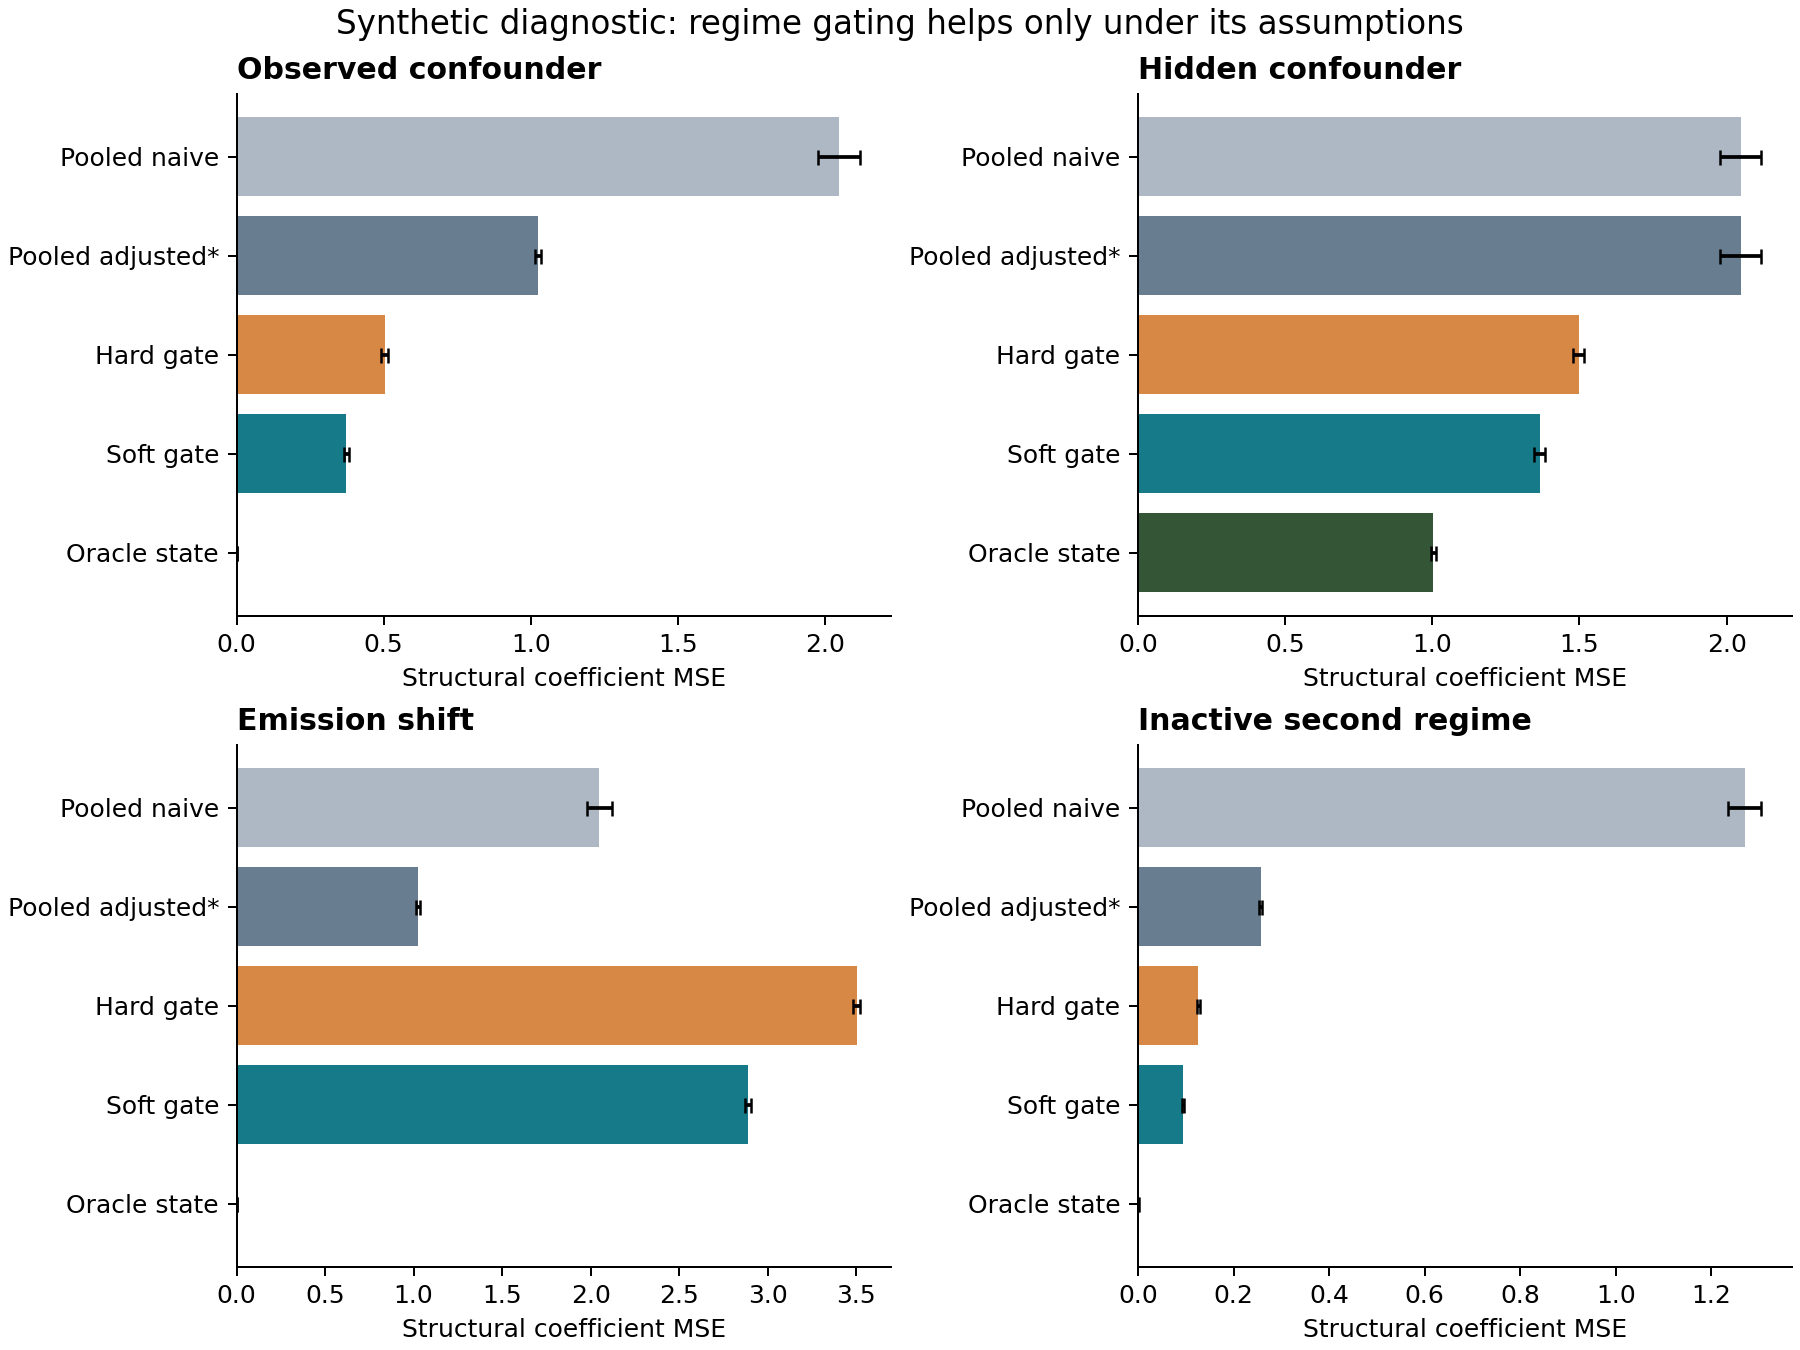
\includegraphics[width=\linewidth]{assets/synthetic_results.png}
\caption{Routing performance depends on both confounding and the validity of the regime observation model. Error bars are 1.96 times the Monte Carlo standard error of mean MSE.}
\end{figure}

\section{Understanding the failure mechanisms}
\subsection{Why oracle regimes do not repair confounding}
Within either regime, $X=C+U$ and $Y=\theta_k X+2C+V$. Independent standard-normal $C,U,V$ give $\operatorname{Var}(X)=2$ and $\operatorname{Cov}(X,C)=1$. Variance measures spread and covariance measures joint variation. The population unadjusted regression slope is therefore
\begin{align}
 \beta_k^{\rm unadjusted}
 &=\frac{\operatorname{Cov}(X,Y\mid S=k)}{\operatorname{Var}(X\mid S=k)}\\
 &=\theta_k+2\frac{\operatorname{Cov}(X,C)}{\operatorname{Var}(X)}
 =\theta_k+1.
\end{align}
We first substitute the outcome equation into covariance, then use independence to remove covariance with $V$, and finally substitute the known variances. The coefficient bias is one, giving squared error one even with perfect state selection and unlimited training data. Finite-sample estimation explains the small departure of the simulated mean from one. This is a property of the declared synthetic model, not a theorem about all hidden-confounder settings.

\subsection{Why probability weighting can help and still fail}
Suppose for this explanation that the state coefficients are known exactly and the filter probabilities are correct. Let $B=\theta_{S_t}$ be the unknown coefficient and $\mathcal{I}_t$ the information available to the filter. For any proposed scalar estimate $a$, write $\bar b=\mathbb{E}[B\mid\mathcal{I}_t]$. Expanding the square gives
\begin{align}
 \mathbb{E}[(B-a)^2\mid\mathcal{I}_t]
 =\operatorname{Var}(B\mid\mathcal{I}_t)+(\bar b-a)^2.
\end{align}
The cross term vanishes because $B-\bar b$ has conditional mean zero. The first term does not depend on $a$, so choosing $a=\bar b=\sum_kq_{t,k}\theta_k$ minimizes conditional squared error. This familiar conditional-mean identity explains soft weighting under its assumptions; estimated coefficients and a misspecified filter need not attain that optimum.

For example, with state coefficients $(1,-1)$ and probabilities $(0.6,0.4)$, soft weighting gives $0.2$. Its conditional MSE is $0.6(1-0.2)^2+0.4(-1-0.2)^2=0.96$. Hard selection gives 1 and MSE $0.4(-1-1)^2=1.6$. If the true coefficient is 1 but a reversed observation model assigns probabilities $(0.1,0.9)$, soft weighting gives $-0.8$ and squared error 3.24. A pooled coefficient near zero then has error near one. Reduced decisiveness helps under uncertainty; incorrect state semantics can dominate that benefit.

\section{Reproducibility and limitations}
All diagnostic data are generated from declared random seeds; no proprietary market data, model API, or accelerator is required. The artifact contains the generator, regressions, filter, router, tests, raw replicate results, and aggregation instructions. Regression design matrices have either two columns (intercept and treatment) or three (also confounder). Each row is one training observation. With this fixed small column count, least-squares work grows approximately linearly with training length. Filtering two states also takes linear time and stores a two-column probability array over the sequence. The reference router passes five contract tests; these tests exercise declared behavior rather than proving economic assumptions.

Training states and nominal filter parameters are oracle inputs. Results therefore isolate specified failure modes and do not establish performance with learned regimes. The evidence router and statistical diagnostic are separate modules: the routing weights from evidence scores are not the filter probabilities used in Table~\ref{tab:cmtf}. No end-to-end experiment combines language-model proposals, graph identification, estimation, regime learning, and trade execution.

The synthetic graph is deliberately simple, with a known treatment effect and independent disturbances. Real economic mechanisms may involve simultaneous feedback, unobserved interventions, revised data vintages, weak support, and multiple plausible graphs. Confidence in a predicted regime is not a calibrated probability that a causal assumption is true. The declaration of identification can itself be wrong; the current router cannot discover that fact.

\section{Conclusion}
CMTF makes the boundary between a proposed mechanism and an eligible decision explicit. Its implemented contribution is a small, inspectable contract for declared evidence; its empirical contribution is a reproducible diagnostic showing how confounding and regime-observation error affect coefficient routing. Under a valid observation model, soft routing improves coefficient recovery. Under hidden confounding, even oracle routing remains biased. Under reversed state semantics, filtered routing becomes worse than pooled adjustment. These outcomes support explicit identification status, provenance, and failure handling, while leaving live economic effectiveness and full neuro-symbolic integration open to separate evaluation.
